\paragraph{}
This appendix presents figures \ref{index_summary} - \ref{question_sample} that show screenshots obtained in a Kibana instance. The purpose of the screenshots is to get an impression of how does exploring the data source indexed in Elasticsearch may look like. A reader is not expected to read the text in the figures.

\begin{figure}[!h]
	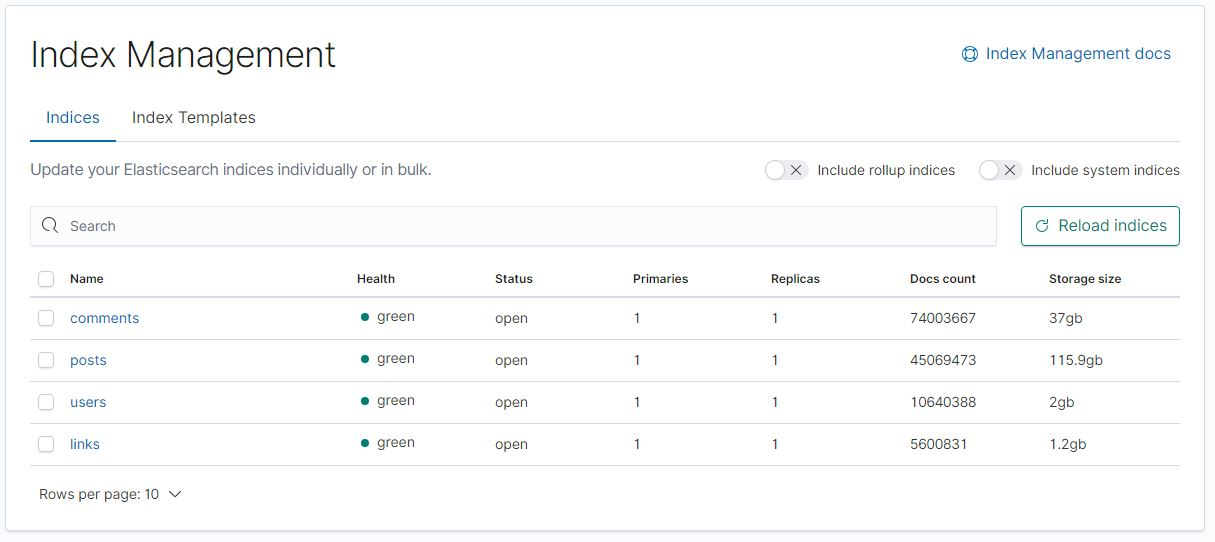
\includegraphics[width=15cm]{index_screenshot.JPG}
	\centering
	\caption{Summary of all documents indexed in the Elasticsearch cluster.}
	\label{index_summary}
\end{figure}

\begin{figure}[!h]
	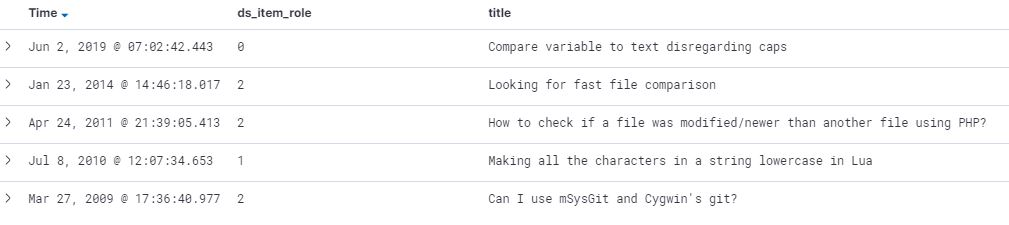
\includegraphics[width=15cm]{ds_item_group.JPG}
	\centering
	\caption{One dataset group displayed in the Kibana instance. The figure shows a master post (\textit{ds\_item\_role = 0}) with a corresponding duplicate (\textit{ds\_item\_role = 1}) and three similar posts (\textit{ds\_item\_role = 2}).}
	\label{ds_item_group}
\end{figure}


\begin{figure}[!h]
	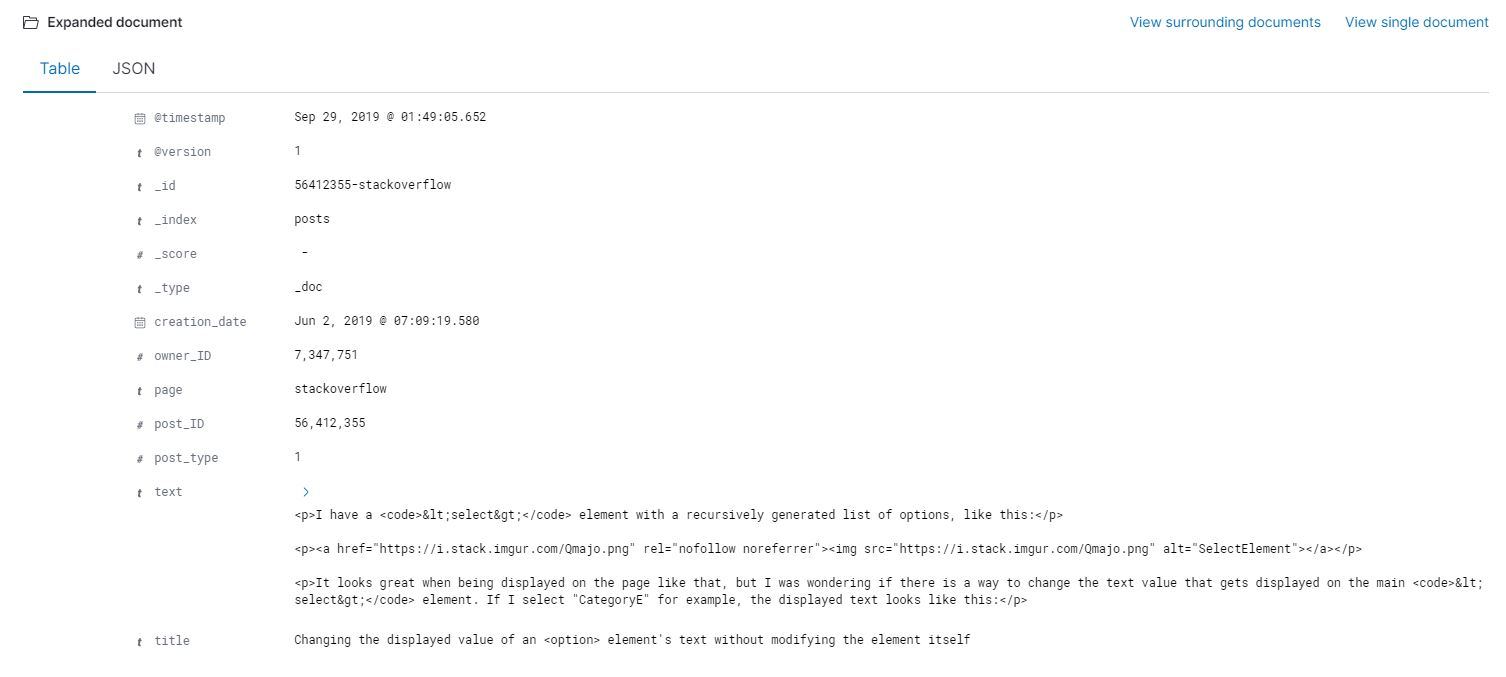
\includegraphics[width=15cm]{es_document_screenshot.JPG}
	\centering
	\caption{Expanded details of one document (post) displayed in the Kibana instance.}
	\label{es_document}
\end{figure}

\begin{figure}[!h]
	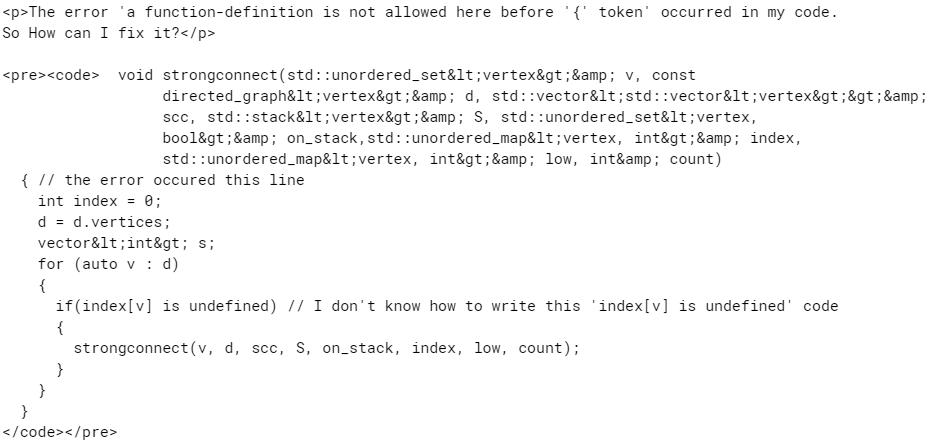
\includegraphics[width=15cm]{question_sample.png}
	\centering
	\caption{Example of an HTML body of one post.}
	\label{question_sample}
\end{figure}